\documentclass[titlepage,german]{scrartcl}
\usepackage{graphicx}
\usepackage[noamsthm]{beamerarticle}
\usepackage[hyphens]{url}
\usepackage[a4paper,head=1.5cm,bottom=2.5cm,left=25mm,right=25mm]{geometry}
\usepackage[colorlinks=true,
        linkcolor=black,
        citecolor=black,
        filecolor=black,
        pagecolor=black,
        urlcolor=black,
        bookmarks=true,
        bookmarksopen=true,
        bookmarksopenlevel=3,
        plainpages=false,
        pdfpagelabels=true]{hyperref}
\usepackage{fancyhdr}
\usepackage{watermark}
\usepackage{scrextend}
\thiswatermark{\put(310,-20){\includegraphics[width=5cm]{blackned_solutions_logo.png}}}
\pagestyle{fancy}
\fancyhf{}
\renewcommand{\headrulewidth}{0pt}
\fancyhead[R]{\includegraphics[height=16px]{blackned.png}}
\fancyfoot[C]{\thepage}
\fancypagestyle{plain}{}
\renewcommand{\headrulewidth}{0.5pt}
\renewcommand{\footrulewidth}{0.5pt}
\pagestyle{fancy}
\usepackage{sectsty}
\usepackage{afterpage}

\chapterfont{\color{Titelfarbe}\selectfont}
\sectionfont{\color{Titelfarbe}\selectfont}
\subsectionfont{\color{Titelfarbe}\selectfont}
\subsubsectionfont{\color{Titelfarbe}\selectfont}

\renewcommand{\labelitemi}{\textcolor{blacknedDarkGray}{$\blacksquare$}}
\renewcommand{\labelitemii}{\textcolor{blacknedMediumGray}{$\circ$}}
\renewcommand{\labelitemiii}{\textcolor{blacknedLightGray}{$\cdot$}}
\renewcommand{\labelitemiv}{\textcolor{blacknedLightGray}{$\ast$}}


\usepackage{helvet}
\renewcommand{\familydefault}{\sfdefault}

\newif\ifshowonlynotes
\showonlynotesfalse


\makeatletter
\newif\ifbeamer@inlecture\beamer@inlecturetrue
\def\beamer@currentmode{beamer}
\input{beamerbasenotes.sty}
\def\beamer@currentmode{article}

\renewcommand\beamer@outsideframenote[2][]{%
  \def\beamer@noteenvstart{}%
  \def\beamer@noteenvend{}%
  \setkeys{beamernotes}{#1}%
  \par
  \beamer@noteenvstart\textit{#2}\beamer@noteenvend%
  \par
}

\setbeamertemplate{frame begin}{\beamer@framenotesbegin}
\setbeamertemplate{frame end}{\beamer@setupnote\beamer@notesactions}

\ifshowonlynotes
  \let\beamer@dosingleframe=\beamer@donoframe
  \g@addto@macro\beamer@endframe{\usebeamertemplate{frame end}}
\fi

\def\note{%
  \ifbeamer@inframe%
    \let\next=\beamer@inframenote%
  \else%
    \par
    \begingroup
      \leftskip=0mm
      \noindent \textbf{Anmerkung:}
      \par
    \endgroup
    \let\next=\beamer@outsideframenote%
  \fi%
  \next}
\makeatother

\makeatletter
\renewenvironment{thebibliography}[1]
     {\@mkboth{\MakeUppercase\bibname}{\MakeUppercase\bibname}%
      \list{\@biblabel{\@arabic\c@enumiv}}%
           {\settowidth\labelwidth{\@biblabel{#1}}%
            \leftmargin\labelwidth
            \advance\leftmargin\labelsep
            \@openbib@code
            \usecounter{enumiv}%
            \let\p@enumiv\@empty
            \renewcommand\theenumiv{\@arabic\c@enumiv}}%
      \sloppy
      \clubpenalty4000
      \@clubpenalty \clubpenalty
      \widowpenalty4000%
      \sfcode`\.\@m}
     {\def\@noitemerr
       {\@latex@warning{Empty `thebibliography' environment}}%
      \endlist}
\makeatother

\makeatletter
\renewcommand\maketitle{
  \linespread{.67}
  \vspace*{8cm}
  \begin{flushleft}
    \Huge\bfseries\textcolor{Titelfarbe}{\@title}
    \textcolor{Titelfarbe}{\rule[1mm]{\linewidth}{.5mm}}
    \huge\bfseries\textcolor{Titelfarbe}{\@subtitle}
  \end{flushleft}
  \linespread{1}
  \pagebreak
}
\makeatother
\usepackage[ngerman]{babel}
\usepackage[T1]{fontenc}
\usepackage[utf8x]{inputenc}
\usepackage{color}
\usepackage{colortbl}
\usepackage{listings}
\usepackage{longtable}
\usepackage{tikz}
\usepackage{amsthm}
\usepackage{amsmath}
\usepackage{pgfplots}
\usetikzlibrary{shapes, calc}
\usetheme[
  outer/progressbar=foot,
  outer/numbering=none
]{metropolis}

\def\datengerman{\def\today{\ifnum\day<10 0\fi\number\day.\ifnum\month<10 0\fi\number\month.\number\year}}
\date{\today}

\newcommand{\befehl}[1]{\ttfamily #1\sf}

\DeclareMathOperator{\e}{e}
\newcommand{\iu}{{\mathrm{i}\mkern1mu}}

\definecolor{SimpsonsYellow}{RGB}{255,217,15}

\setbeamercolor{progress bar in head/foot}{fg=SimpsonsYellow}
\setbeamercolor{title separator}{fg=SimpsonsYellow}
\setbeamercolor{frametitle}{fg=black,bg=SimpsonsYellow}

\title{The Simpsons meet IT}
\subtitle{Was wir von den Simpsons und Futurama über Mathematik, Kryptografie, IT und Quantenphysik lernen können}


\only<article>{
  \publishers{\textcopyright\ Markus Flingelli, 2016 - \the\year}
}

\only<article>{
  \hypersetup{
  pdftitle = {The Simpsons meet IT -- Was wir von den Simpsons und Futurama über Mathematik, Kryptografie, IT und Quantenphysik lernen können},
  pdfsubject = {},
  pdfkeywords = {Simpsons, IT, Mathematik, Informatik, Physik},
  pdfauthor = {\textcopyright\ Markus Flingelli, 2016 - \the\year},
  pdfcreator = {\LaTeX\ u.a. mit dem Paket \flqq hyperref\frqq},
  pdfproducer = {pdfeTeX-0.\the\pdftexversion\pdftexrevision},
  }
}

\hypersetup{colorlinks=true, linkcolor=black, urlcolor=blue}

\definecolor{Titelfarbe}{RGB}{245,255,250}
\definecolor{Titelhintergrundfarbe}{RGB}{255,217,15}
\definecolor{ivory}{RGB}{255,255,240}
\definecolor{basicGreen}{RGB}{0,140,0}
\definecolor{basicRed}{RGB}{128,0,0}

\theoremstyle{plain}
\newtheorem{lem}{Lemma}

\lstdefinestyle{base}{
  language={[Visual]Basic},
  emptylines=1,
  breaklines=true,
  basicstyle=\ttfamily\color{basicRed},
  moredelim=**[is][\color{basicGreen}]{@}{@},
}

\AtBeginSection[]
{
  \begin{frame}<beamer>
    \frametitle{Gliederung}
    \tableofcontents[sections={\thesection}]
  \end{frame}
  \begin{frame}<handout>
    \frametitle{Gliederung}
    \tableofcontents[sections={\thesection}]
  \end{frame}
}
\setlength\parindent{0pt}
\KOMAoptions{twoside=true}

\xdef\Colored{1}
\ifnum\Colored > 0
\xdef\LWS{0.6mm}
\xdef\ColorYO{yellow!30!orange}
\xdef\ColorYR{yellow!70!red}
\xdef\ColorRY{red!90!yellow}
\xdef\ColorYB{yellow!90!brown}
\xdef\ColorYRB{yellow!90!red}
\xdef\ColorR{red}
\xdef\ColorO{orange}
\else
\xdef\LWS{0.4mm}
\xdef\ColorYO{gray!80!black}
\xdef\ColorYR{gray!70}
\xdef\ColorRY{gray!60!black}
\xdef\ColorYB{gray!90}
\xdef\ColorYRB{gray!50}
\xdef\ColorR{black}
\xdef\ColorO{gray!95!black}
\fi
\newenvironment{enuma}{\begin{enumerate}[label={\alph{enumi})}, itemsep=-1mm]}{\end{enumerate}}
\newlength\tipWidth
\newlength\tipSeparator
\newlength\tipTextWidth
\newlength\addedWidth
\newlength\addedHeight
\newlength\RectHeight
\newlength\testL
\newlength\lengthA
\newlength\lengthB
\newlength\lengthC
\setlength\addedHeight{3mm}
\setlength\addedWidth{4mm}
\setlength\tipSeparator{6mm}
\newsavebox{\lambBox}
\newsavebox{\lambVBox}
\newsavebox{\tipBox}
\newsavebox{\tipVBox}
\newcommand{\Hinweis}[4][\tipWidth]{%
\def\alig{#2}%
\def\aligm{m}%
\def\aligt{t}%

\savebox{\lambBox}{\hbox{\begin{tikzpicture}[inner sep=0,outer sep=0]
\fill[rounded corners=0.35mm,rotate=-15,gray!90!black] (0.05,-0.15)rectangle(-0.1,-0.02);
\draw[line width=0.9mm] (0.2,0.01) to[in=330 , out=170] (-0.2,0.11);
\draw[line width=1mm] (0.3,0.15) to[in=330 , out=170] (-0.25,0.25);
\draw[line width=1.1mm] (0.35,0.3) to[in=350 , out=180] (-0.27,0.36);
\draw[line width=\LWS, color=\ColorYO] (-0.15,0.42) to[in=310,out=80] (-0.3,0.8)to[in=215,out=130](-0.37,1.15) to[out=45,in=150] (0.2,1.35)to[in=110,out=-30](0.56,0.99)to[in=45,out=290](0.41,0.69)to[in=80,out=215](0.2,0.37);
\draw[line width=0.2mm] (0.,0.33)--(-0.02,0.72);
\fill[\ColorYR] (-0.02,0.72)--(0.0,0.93)--(0.055,0.79)--(0.07,0.9)--(0.13,0.79)--(0.28,0.8)--(0.16,0.61)--(0.09,0.65)--(0.07,0.5)--(0.046,0.54)--cycle;
\fill[\ColorRY] (-0.02,0.72)--(0.008,0.78)--(0.05,0.68)--(0.07,0.84)--(0.15,0.74)--(0.28,0.8)--(0.165,0.69)--(0.10,0.74)--(0.07,0.63)--(0.045,0.63)--(0.015,0.72)--cycle;
\draw[line width=0.2mm] (0.02,0.3)--(0.28,0.8);
\draw[line width=0.7mm,\ColorYB](0.25,1.46)--(0.32,1.69) (0.41,1.33)--(.61,1.57) (0.54,1.19)--(.7,1.33) (0.03,1.5)--(-0.0,1.8) (-0.18,1.42)--(-0.3,1.62) (-0.4,1.3)--(-0.58,1.49);
\draw[line width=0.3mm,\ColorYRB] (-0.3,1.05)to[in=120,out=20](0.5,0.96);
\end{tikzpicture}}}%
\savebox\lambVBox{\vbox{\usebox{\lambBox}}}%
\setlength\tipTextWidth{0 pt}%
\addtolength\tipTextWidth{#1}%
\addtolength\tipTextWidth{-\wd\lambBox}%
\addtolength\tipTextWidth{-\tipSeparator}%
\addtolength\tipTextWidth{-\addedWidth}%
\addtolength\tipTextWidth{-\addedWidth}%
\savebox{\tipBox}{\hbox{\begin{minipage}[inner sep=0,outer sep=0]{\tipTextWidth}{\noindent\bfseries #3} #4\end{minipage}}}%
\savebox{\tipVBox}{\vbox{\usebox{\tipBox}}}%
\setlength\testL{\ht\tipVBox}%
\addtolength\testL{\dp\tipVBox}%
\addtolength\testL{-\ht\lambBox}%
\addtolength\testL{-\dp\lambBox}%
\setlength\lengthA{\ht\tipVBox}%
\addtolength\lengthA{-0.5\ht\lambBox}%
\setlength\lengthB{0.5\ht\lambBox}%
\addtolength\lengthB{-\ht\tipVBox}%
\setlength\lengthC{0.5\ht\tipVBox}%
\addtolength\lengthC{0.5\dp\tipVBox}%
\begin{tikzpicture}[inner sep=0, outer sep =0]%
\node[inner sep=0,outer sep=0] at ({-0.5\wd\lambBox-0.5\tipSeparator},{\ifx\alig\aligm 0\else \ifdim\testL > 0pt \lengthA\else 0\fi\fi}) {\usebox{\lambBox}};
\node[inner sep=0,outer sep =0] at ({0.5\tipTextWidth+0.5\tipSeparator},{\ifx\alig\aligm 0\else \ifdim\testL > 0pt 0\else \lengthB\fi\fi}) {\usebox{\tipBox}};
\draw[\ColorO,line width=0.5mm] (0,\ifdim\testL> 0pt -\ht\tipVBox \else -0.5\ht\lambBox\fi)--(0,\ifdim\testL> 0pt \lengthC \else 0.5\ht\lambBox\fi);
\end{tikzpicture}%

}

\usepackage[ngerman]{babel}
\usepackage[T1]{fontenc}
\usepackage[utf8x]{inputenc}
\usepackage{color}
\usepackage{colortbl}
\usepackage{listings}
\usepackage{longtable}
\usepackage{tikz}
\usepackage{amsthm}
\usepackage{amsmath}
\usepackage{pgfplots}
\usetikzlibrary{shapes, calc}
\usetheme[
  outer/progressbar=foot,
  outer/numbering=none
]{metropolis}

\makeatletter
\setlength{\metropolis@titleseparator@linewidth}{2pt}
\setlength{\metropolis@progressonsectionpage@linewidth}{2pt}
\setlength{\metropolis@progressinheadfoot@linewidth}{2pt}
\makeatother

\definecolor{SimpsonsYellow}{RGB}{255,217,15}

\setbeamercolor{progress bar in head/foot}{fg=SimpsonsYellow}
\setbeamercolor{title separator}{fg=SimpsonsYellow}
\setbeamercolor{frametitle}{fg=black,bg=SimpsonsYellow}

\title{The Simpsons meet IT}
\subtitle{Was wir von den Simpsons und Futurama über Mathematik, Kryptografie, IT und Quantenphysik lernen können}
\author{ Dipl.-Inform. (univ.) Markus M. Flingelli}

\only<article>{
  \publishers{\textcopyright\ Markus Flingelli, 2016 - \the\year}
}

\def\datengerman{\def\today{\ifnum\day<10 0\fi\number\day.\ifnum\month<10 0\fi\number\month.\number\year}}
\date{\today}

\hypersetup{colorlinks=true, linkcolor=black, urlcolor=blue}

\definecolor{ivory}{RGB}{255,255,240}
\definecolor{basicGreen}{RGB}{0,140,0}
\definecolor{basicRed}{RGB}{128,0,0}
\newcommand{\befehl}[1]{\ttfamily #1\sf}

\theoremstyle{plain}
\newtheorem{lem}{Lemma}

\DeclareMathOperator{\e}{e}
\newcommand{\iu}{{\mathrm{i}\mkern1mu}}

\lstdefinestyle{base}{
  language={[Visual]Basic},
  emptylines=1,
  breaklines=true,
  basicstyle=\ttfamily\color{basicRed},
  moredelim=**[is][\color{basicGreen}]{@}{@},
}

\AtBeginSection[]
{
  \begin{frame}<beamer>
    \frametitle{Gliederung}
    \tableofcontents[sections={\thesection}]
  \end{frame}
  \begin{frame}<handout>
    \frametitle{Gliederung}
    \tableofcontents[sections={\thesection}]
  \end{frame}
}

\begin{document}

\only<article>{
  \thispagestyle{empty}
  \pagecolor{black}\afterpage{\nopagecolor}
  \maketitle
}

\frame{\titlepage}

\frame{
\only<presentation>{
  \frametitle{Inhaltsverzeichnis}
}
\tableofcontents[hideallsubsections]
}
\only<article>{
  \newpage
}

\section{Linux}

\begin{frame}[fragile]
\only<presentation>{
	\frametitle{Linux}
}
\begin{block}{Hölle, Tod und Geister}
\begin{lstlisting}[language=Bash]
cat westerbrook > /dev/null
\end{lstlisting}
\end{block}
\end{frame}
\note{
Halloween-Folge der 26. Staffel (Treehouse of Horror XXV)
}

\section{Mathematik}

\subsection{Zahlentheorie}

\begin{frame}
\frametitle{Das sollten wir nicht lernen!}
\begin{figure}[ht]
	\centering
	\only<presentation>{
		
\includegraphics[width=.65\textwidth]{frink_pi.png}
	}
	\only<article>{
	  
\includegraphics[width=.75\textwidth]{frink_pi.png}
	}
\end{figure}
\scriptsize{Quelle: \href{https://tstoaddicts.files.wordpress.com/2014/03/frink-pi.jpg}{\url{https://tstoaddicts.files.wordpress.com/2014/03/frink-pi.jpg}}}
\end{frame}

\note{
\begin{itemize}
	\item Dr. Edmund Stoiber gibt an, im deutschen Fernsehen gebe es \glqq nur noch kaputte Familien. Außer den Simpsons gibt es keine normale Familie mehr im TV \cite{FIS}.\grqq
	\item Universität von Glasgow in Schottland bietet ein Seminar mit dem Titel \glqq D'Oh! The Simpsons Introduce Philosophy\grqq\ an (Matt Groening hat Philosophie studiert) \cite{BBC}
	\item Simpsons- und Futurama haben teilweise naturwissenschaftlichen Hintergrund:
	\begin{itemize}
		\item Jeff Westerbrook:
		\begin{itemize}
		  \item Bachelorabschlüsse in Physik und Wissenschaftsgeschichte
		  \item Promotion im Bereich theoretischer Informatik
		  \item War als Forscher an der Yale University tätig
		  \item Erd\H{o}s-Zahl: 3
		\end{itemize}
		\item David X. Cohen: Bachelorabschluss in Physik und Masterabschluss in Informatik
		\item Ken Keeler:
		\begin{itemize}
		  \item Bachelorabschluss in angewandter Mathematik 
		  \item Masterabschluss in Elektrotechnik
		  \item Promotion in angewandter Mathematik
		  \item Erd\H{o}s-Zahl: 4
		\end{itemize}
		\item Bill Ordenkirk: Promotion im Bereich anorganische Chemie
		\item J. Stewart Burns: Masterabschluss in Mathematik
		\item Al Jean: Bachelorabschluss in Mathematik
	\end{itemize}
\end{itemize}
}

\begin{frame}
\frametitle{Kreiszahl $\pi$}
\begin{itemize}
	\item Wer wird Millionär?
	\begin{itemize}
		\item $\pi$th Avenue
	\end{itemize}
	\item Marge wird verhaftet
	\begin{itemize}
		\item Apu kennt die ersten 40.000 Nachkommastellen von $\pi$
		\item Die 40.000ste Nachkommastelle lautet $1$
	\end{itemize}
	\item Ein bekanntes Möbelhaus: $\pi\mbox{KEA}$
\end{itemize}
\end{frame}

\note{
Datei mit der ersten Million Nachkommastellen von $\pi$: \href{http://www.aip.de/~wasi/PI/Pibel/pibel_10mio.pdf}{\url{http://www.aip.de/~wasi/PI/Pibel/pibel\_10mio.pdf}}
}

\frame{
\only<presentation>{
	\frametitle{Zahlen}
}
\begin{block}{}
\begin{itemize}
	\item Im Reich der Parasiten
	\begin{itemize}
		\item Aus der Route 66 wurde die Historic $\sqrt{66}$
	\end{itemize}
	\item Homer auf Abwegen
	\begin{align*}
		10^{100} &= \mbox{Googol}\\
		10^{\text{Googol}} &= 10^{10^{100}} = \mbox{Googolplex}
	\end{align*}
	\item Dieses unheimliche Hupen
	\begin{itemize}
		\item Bender sieht im Spiegel die mit Blut geschriebene Binärzahl $0101100101$
		\item Gespiegelt: $1010011010_2 = 666_{10}$
	\end{itemize}
\end{itemize}
\end{block}
}

\note{
\begin{itemize}
	\item Googol
	\begin{itemize}
		\item $10^{100} < 70!$
		\item Anzahl der Atome im Universum zwischen $10^{84}$ und $10^{89}$
	\end{itemize}
	\item Weitere Referenzen von Googolplex
	\begin{itemize}
		\item Der Name des Firmenhauptsitzes von Google lautet Googleplex in Anlehnung an den Googolplex.
		\item Im Film Zurück in die Zukunft III nennt Dr. Brown die Chance seine Frau zu treffen 1 zu Googolplex.
		\item In einem Peanuts-Comic erklärt Schroeder seiner Verehrerin Lucy, dass die Chancen für ihre Heirat 1 zu Googol stehen.
	\end{itemize}
\end{itemize}
}

\frame{
\frametitle{Exkurs: Belphegors Primzahl}
\begin{block}{Definition:}
Folgende Zahl, wird als Belphegors Primzahl bezeichnet:
\[1\underbrace{0000000000000}_{\mbox{13 Ziffern}}666\underbrace{0000000000000}_{\mbox{13 Ziffern}}1
\]
\end{block}
}

\note{
\begin{itemize}
	\item Als Dämon fand Belphegor Eingang in die christliche Mythologie (ursprüngliche moabitische Gottheit)
	\item In der italienischen Renaissance erscheint Belphegor in einer Novelle des Niccol\`{o} Machiavelli
	\begin{itemize}
		\item Höllenfürst Pluto bemerkt, dass viele der in der Hölle eintreffenden Männerseelen ihre Ehefrauen für ihre Verdammnis verantwortlich machen.
		\item Er beruft eine Versammlung ein, die beschließt, den ehemaligen Erzengel und jetzigen Erzteufel Belfagor mit der Untersuchung des Phänomens \glqq Ehe\grqq\ zu beauftragen.
		\item Der begibt sich in Gestalt eines Roderigo von Kastilien mit 100.000 Dukaten in der Tasche nach Florenz, wo er auch schon schnell eine ehewillige Dame namens Onesta Donati findet.
		\item Bald schon ist Don Roderigos Vermögen durch Eitelkeit und Putzsucht seiner Frau und die Raffgier ihrer Verwandten zerronnen.
		\item Er wird von Gläubigern und Bütteln verfolgt und kann sich nur knapp vor dem Schuldgefängnis heim in die Hölle retten.
	\end{itemize}
\end{itemize}
}

\frame{
\frametitle{Zahlen}
\begin{block}{Futurama}
\begin{itemize}
	\item Seriennummer von Bender Bending Rodriguez, Sr. (auch bekannt als Bending Unit 22):
		\[2.716.057
	\]
	\item Seriennummer von Flexo:
		\[3.370.318
	\]
	\item Bender and Flexo share their serial numbers:  \href{https://youtu.be/WUH0-Z19JQs}{\url{https://youtu.be/WUH0-Z19JQs}}
\end{itemize}
\end{block}
}

\frame{
\frametitle{Natürliche Zahlen als Summe von Kubikzahlen}
\begin{block}{Definition:}
Natürliche Zahl $n$, die sich als Summe zweier Kubikzahlen darstellen lässt.
\end{block}
\begin{block}{Beispiele:}
\begin{align*}
	3.370.318 &= 119^3 + 119^3\\
	2.716.057 &= 952^3 + (-951)^3
\end{align*}
\end{block}
}

\frame{
\only<presentation>{
	\frametitle{Zahlen}
}
\begin{block}{Homerun für die Liebe}
\begin{itemize}
	\item Besucher sollen Anzahl der Stadionbesucher schätzen
	\item Zur Auswahl stehen folgende drei Zahlen
	\begin{itemize}
		\item $8128$
		\item $8208$
		\item $8191$
	\end{itemize}
\end{itemize}
\end{block}
}

\frame{
\frametitle{Vollkommene Zahlen}
\begin{block}{Definition:}
Die Summe ihrer Teiler ist die Zahl selbst.
\end{block}
\begin{block}{Erste vier vollkommene Zahlen:}
\begin{align*}
	6 = 1 &+ 2 + 3\\
	28 = 1 &+ 2 + 4 + 7 + 14\\
	496 = 1 &+ 2 + 4 + 8 + 16 + 31 + 62 + 124 + 248\\
	8128 = 1 &+ 2 + 4 + 8 + 16 + 32 + 64 + 127 + 254 + 508 + 1016\\
	&+ 2032 + 4064
\end{align*}
\end{block}
}

\frame{
\frametitle{Narzisstische Zahl}
\begin{block}{Definition:}
Summe ihrer Ziffern, jeweils potenziert mit der Stellenanzahl der Zahl, ergibt wieder die Zahl selbst.
\end{block}
\begin{block}{Beispiel:}
\[8^4 + 2^4 + 0^4 + 8^4 = 8208\]
\end{block}
}

\frame{
\frametitle{Mersenne-Primzahl}
\begin{block}{Definition:}
Zahl der Form $2^p - 1$ mit $p$ ist Primzahl.
\end{block}
\begin{block}{Beispiel:}
\[2^{13} - 1 = 8191\]
\end{block}
}

\frame{
\frametitle{Der Da-Blödi-Code}
\begin{block}{Vermeintliche Mersenne-Primzahl:}
$2047$ ist die kleinste Zahl des Typs $2^p - 1$, die keine Primzahl ist.
\begin{align*}
	\mbox{II}^{\mbox{XI}} - \mbox{(XXIII} \cdot \mbox{LXXXIX)} &= 2^{11} - (23 \cdot 89)\\
	2^{11} - (23 \cdot 89) &= 1\\
	2^{11} - 1 &= 2047
\end{align*}
\end{block}
}

\frame{
\frametitle{Kleiner Satz des Fermat}
\begin{block}{Simpsorama}
\begin{itemize}
	\item Auf Innenseite des Deckels in Benders Kopf steht:
		\[
		a^{p-1} \equiv 1\pmod p
	\]
	\item Allgemein gültige Kongruenz lautet:
				\[
		a^p \equiv a\pmod p
	\]
\end{itemize}
\end{block}
}

\frame{
\frametitle{Kongruenz}
\begin{block}{Definition:}
Zwei Zahlen $a$ und $b$ heißen kongruent modulo $m$, wenn $m$ die Differenz $a - b$ teilt
\begin{align*}
	a &\equiv b\mod m\\
	a &\equiv b\mod m\mathbb{Z}\\
	a &\equiv b\pmod {m}\\
	&\Leftrightarrow m|(a-b)\\
	&\Leftrightarrow \exists k \in \mathbb{Z}: a = km + b
\end{align*}
\end{block}
}

\frame{
\frametitle{Kongruenz}
\begin{block}{Beispiele:}
\begin{align*}
	7 &\equiv 3\mod 4\\
	&\Leftrightarrow 4|(7-3)
\end{align*}
\begin{align*}
	27 &\equiv 11\mod 4\\
	&\Leftrightarrow 4|(27-11)
\end{align*}
\begin{align*}
	2^{3-1} &\equiv 1\mod 3\\
	&\Leftrightarrow 3|(2^{3-1} - 1)
\end{align*}
\end{block}
}

\frame{
\frametitle{Hardy-Ramanujan-Zahl}
\begin{block}{Xmas Story}
\begin{itemize}
	\item Bender erhält zu Weihnachten Karte von Mom
	\item Der Text auf der Karte lautet: \textit{MERRY XMAS SON \#1729}
	\item Registernummer der Nimbus, des Raumschiffs von 25-Sterne General Zapp Brannigan ist 1729
\end{itemize}
\end{block}
}

\note{
\begin{itemize}
	\item Name geht auf Anekdote von Godfrey Harold Hardy zurück (siehe \cite{ZOT})
	\item Hardy besuchte Ramanujan am Krankenbett und erwähnte, dass er mit einem Taxi mit der Nummer 1729 gekommen sei
	\item Hardy fand, dies sei eine uninteressante Zahl
	\item Ramanujan widersprach ihm
\end{itemize}
}

\frame{
\frametitle{Hardy-Ramanujan-Zahl}
\begin{block}{Definition:}
Kleinste natürliche Zahl, für die es genau zwei Darstellungen als Summe zweier positiver Kubikzahlen gibt:
\begin{align*}
	9^3 + 10^3 &= 1729\\
	1^3 + 12^3 &= 1729
\end{align*}
\end{block}
}

\frame{
\frametitle{Sphenische Zahl}
\begin{block}{Definition:}
Produkt von genau drei verschiedenen Primzahlen
\end{block}
\begin{block}{Beispiel:}
\[1729 = 7 \cdot 13 \cdot 19\]
\end{block}
}

\note{$1729$ ist das Produkt der ersten drei fröhlichen Primzahlen.}

\frame{
\frametitle{Harshad-Zahl}
\begin{block}{Definition:}
\begin{itemize}
  \item Auch als Niven-Zahl bekannt
  \item Zahl ist durch ihre Quersumme ganzzahlig teilbar
\end{itemize}
\end{block}
\begin{block}{Beispiel:}
\[
(1 + 7 + 2 + 9)\cdot 91 = 1729
	\]
\end{block}
}

\note{
\begin{itemize}
  \item Der Begriff Harshad-Zahl wurde vom indischen Mathematiker D. R. Kaprekar eingeführt und ist vom Sanskrit-Wort \textit{harsha} (\glqq Freude\grqq ) abgeleitet.
  \item Die Niven-Zahl geht auf den Mathematiker Ivan M. Niven zurück, der diese Zahlen an einem Kongress im Jahre 1997 beschrieb.
\end{itemize}
}

\frame{
\frametitle{Carmichael-Zahl}
\begin{block}{Definition:}
Eine zusammengesetzte natürliche Zahl $n$ heißt Carmichael-Zahl, falls für alle zu $n$ teilerfremden Zahlen $a$ die folgende Kongruenz erfüllt ist:
\[
	a^{n-1} \equiv 1 \mod n
\]
\end{block}
\begin{block}{Beispiel:}
\[
	a^{1728} \equiv 1 \pmod{1729}
\]
\end{block}
}

\note{
\begin{itemize}
  \item Carmichael-Zahlen haben mindestens drei Primfaktoren.
  \item Es gibt unendlich viele Carmichael-Zahlen.
  \item Benannt nach dem US-amerikanischen Mathematiker Robert Daniel Carmichael.
\end{itemize}
}


\frame{
\frametitle{Eulersche Pseudoprimzahl}
\begin{block}{Definition:}
Eine ungerade zusammengesetzte natürliche Zahl $n$ heißt eulersche Pseudoprimzahl zur Basis $a$, wenn
\begin{align*}
	a^{\frac{n-1}{2}} \equiv \pm 1 \mod n\\
\end{align*}
gilt.
\end{block}
}

\frame{
\frametitle{Absolute eulersche Pseudoprimzahlen}
\begin{block}{Definition:}
\begin{itemize}
  \item Zahlen $n$, die zu allen teilerfremden Basen $a$ eine eulersche Pseudoprimzahl darstellen, nennt man absolute eulersche Pseudoprimzahlen.
  \item Kleinste absolute eulersche Pseudoprimzahl: $1729$
\end{itemize}
\end{block}
}

\frame{
\frametitle{Eulersche Zahl}
\begin{block}{Definition:}
\begin{itemize}
	\item Eulersche Zahl $e = 2,71828...$
	\item Irrational und transzendente reelle Zahl
	\item Basis des natürlichen Logarithmus und der natürlichen Exponentialfunktion
	\item An 1729. Nachkommastelle treten erstmals die Ziffern $0$ bis $9$ hintereinander auf
\end{itemize}
\begin{align*}
	e = 2,71828...58897\underbrace{0719425863}_{}987727...\\
\end{align*}
\end{block}
}

\frame{
\frametitle{Transzendente Zahl}
\begin{block}{Definition:}
\begin{itemize}
	\item Reelle Zahl ist transzendent, wenn sie nicht Nullstelle eines (vom Nullpolynom verschiedenen) Polynoms mit ganzzahligen Koeffizienten ist.
	\item Jede transzendente Zahl ist überdies irrational.
\end{itemize}
\end{block}
}

\note{Eine reelle Zahl heißt irrational, wenn sie nicht als Bruch zweier ganzer Zahlen dargestellt werden kann; sie kann nicht als $\frac{p}{q}$ mit $p$, $q \in \mathbb{Z}$ und $q \neq 0$ geschrieben werden.}

\begin{frame}
\only<article>{
  \newpage
}
\frametitle{Bender's Big Score}
\begin{block}{Taxicab-Zahl}
Fry ruft Taxi mit der Nummer $87.539.319$

\end{block}
\begin{figure}[ht]
	\centering
	\only<presentation>{
	  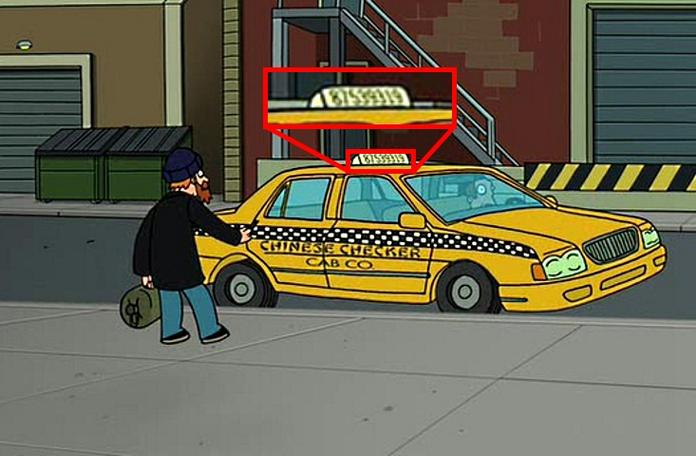
\includegraphics[width=.6\textwidth]{taxi_futurama.png}
	}
	\only<article>{
	  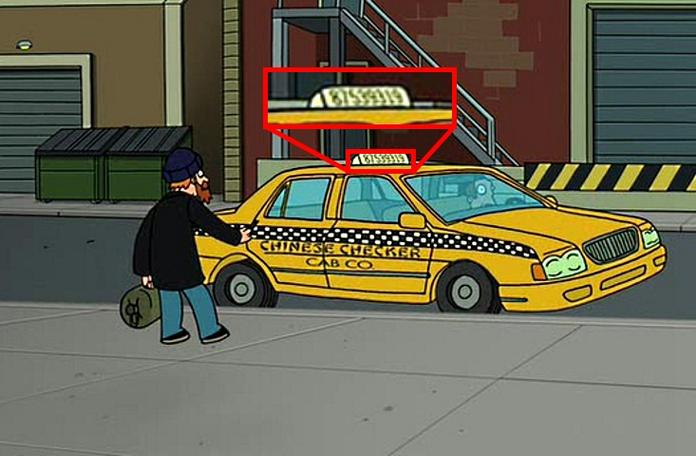
\includegraphics[width=.8\textwidth]{taxi_futurama.png}
	}
\end{figure}
\scriptsize{Quelle: \href{https://1.f.ix.de/scale/geometry/696x500/q75/imgs/71/2/0/3/8/7/9/9/taxi-9af2d4242b8b6510.jpg}{\url{https://1.f.ix.de/scale/geometry/696x500/q75/imgs/71/2/0/3/8/7/9/9/taxi-9af2d4242b8b6510.jpg}}}
\end{frame}

\frame{
\only<presentation>{
  \frametitle{Taxicab-Zahl}
}
\begin{block}{Definition:}
Kleinste natürliche Zahl $n$, die sich auf $n$ verschiedene Arten als Summe zweier Kubikzahlen darstellen lässt:
\begin{align*}
	Ta(1) &= 2           &&= 1^3 + 1^3\\
	Ta(2) & = 1729       && = 1^3 + 12^3\\
	      &              && = 9^3 + 10^3\\
	Ta(3) & = 87.539.319 && = 167^3 + 436^3\\
	      &              && = 228^3 + 423^3\\
	      &              && = 255^3 + 414^3
\end{align*}
\end{block}
}


\frame{
\frametitle{Großer Satz des Fermat}
\begin{block}{Im Schatten des Genies}
\begin{itemize}
	\item Homer schriebt vermeintliches Gegenbeispiel an die Tafel:
		\[
		3987^{12} + 4365^{12} = 4472^{12}
	\]
	\item In der Episode \emph{Die Panik-Amok-Horror-Show} erscheint folgende Gleichung:
		\[
		1782^{12} + 1841^{12} = 1922^{12}
		\]
\end{itemize}
\end{block}
}

\note{
\begin{itemize}
  \item Episoden geschrieben von David X. Cohen.
  \item Schrieb C-Programme, um Werte zu finden, die Gleichung beim Eintippen in herkömmliche Taschenrechner scheinbar lösen.
\end{itemize}
}

\frame{
\only<presentation>{
  \frametitle{Großer Satz des Fermat}
}
\begin{block}{Definition:}
Sei $n > 2$ eine natürliche Zahl, dann gibt es keine von Null verschiedenen natürlichen Zahlen $x$, $y$ und $z$ mit
		\[
		x^n + y^n = z^n
	\]
\end{block}
}

\note{
\begin{itemize}
  \item Pierre de Fermat war Jurist.
  \item 1640 schrieb er als Randnotiz in einem Buch, dass er einen Beweis gefunden habe.
  \item Endgültig bewiesen durch Andrew Wiles 1994 (siehe \cite{BOE}).
  \item Wiles las als Zehnjähriger erstmals in einem Buch von diesem Problem und war fasziniert von diesem Problem.
\end{itemize}
}

\subsection{Geometrie}

\frame{
\frametitle{Eulersche Formel}
\begin{block}{The Lisa Series}
\begin{itemize}
	\item Lisa liest ein Buch mit folgendem Titel:
\end{itemize}
	\[\e^{\iu\pi} + 1 = 0\]
\end{block}
}

\frame{
\only<presentation>{
  \frametitle{Eulersche Formel}
}
\begin{block}{Definition:}
\begin{itemize}
	\item Die eulersche Formel bezeichnet die für $y\in \mathbb {R}$ gültige Gleichung
\end{itemize}
	\[\e^{\iu y} = cos(y) + \iu sin(y)\]
	\begin{itemize}
	\item Für $y = \pi$ ergibt sich aus der eulerschen Formel die sogenannte eulersche Identität
\end{itemize}
	\begin{align*}
		\e^{\iu\pi} &= -1\\
		\e^{\iu\pi} + 1 &= 0
	\end{align*}
\end{block}
}

\frame{
\frametitle{Verallgemeinerung des Satzes des Pythagoras}
\begin{block}{Vom Teufel besessen}
\begin{itemize}
	\item Homer behauptet:
\end{itemize}
\begin{quotation}
	\glqq Die Summe der Quadratwurzeln der beiden Seiten eines gleichschenkligen Dreiecks entspricht der Quadratwurzel der verbliebenen Seite.\grqq
\end{quotation}

\begin{minipage}{0.35\textwidth}
	\begin{center}
	\only<presentation>{
	\begin{tikzpicture}[scale=.5, every node/.style={scale=.5}]
	}
	\only<article>{
	\begin{tikzpicture}[scale=.75, every node/.style={scale=.75}]
	}
		\coordinate (A) at (0,0);
\coordinate (B) at (4,0);
\coordinate (C) at (2,3.464);

\coordinate[label=below:$b$](c) at ($ (A)!.5!(B) $);
\coordinate[label=left:$a$] (b) at ($ (A)!.5!(C) $);
\coordinate[label=right:$a$](a) at ($ (B)!.5!(C) $);

% angle alpha
\draw[fill=green!30] (0,0) -- (0:0.75cm) arc (0:60:.75cm);
\draw (0.35cm,0.25cm) node {$\alpha$};

% angle beta
\begin{scope}[shift={(4cm,0cm)}]
	\draw[fill=green!30] (0,0) -- (-180:0.75cm) arc (180:120:0.75cm);
	\draw (150:0.5cm) node {$\beta$};
\end{scope}

% angle gamma
\begin{scope}[shift={(60:4)}]
	\draw[fill=red!30] (0,0) -- (-120:.75cm) arc (-120:-60:.75cm);
	\draw (-90:0.5cm) node {$\gamma$};
\end{scope}


\draw [line width=.5pt] (A) -- (B) -- (C) -- cycle;

	\end{tikzpicture}
	\end{center}
\end{minipage}
\hfill
\begin{minipage}{0.6\textwidth}
	\begin{align}
		\sqrt{a} + \sqrt{a} &= \sqrt{b}\\
		\sqrt{a} + \sqrt{b} &= \sqrt{a}
	\end{align}
\end{minipage}
\end{block}
}

\note{
\begin{itemize}
	\item Beweis durch Widerspruch
	\item Sei $a = 9$ und $b = 4$
\end{itemize}
\begin{align*}
	\sqrt{9} + \sqrt{9} &\neq \sqrt{4}\\
	\sqrt{9} + \sqrt{4} &\neq \sqrt{9}
\end{align*}
}

\subsection{Mengenlehre}

\frame{
\frametitle{Aleph-Funktion}
\begin{block}{Definition:}
\begin{itemize}
	\item Aufzählung aller unendlichen Kardinalzahlen
	\item Rekursive Definition:
\end{itemize}
\begin{align*}
	\aleph_0 &= \mbox{kleinste unendliche Kardinalzahl}\\
	\aleph_{\alpha +1} &= \mbox{kleinste Kardinalzahl, die größer als}\ \aleph_0\ \mbox{ist}\\
	\aleph_{\alpha} &= \sup \left\{\aleph_{\beta}\mbox{;}\ \beta \le \alpha \right\} \mbox{für Limes-Ordinalzahlen}\ \alpha
\end{align*}
\end{block}
}

\frame{
\only<presentation>{
	\frametitle{Aleph-Funktion}
}
\begin{block}{Beispiele:}
\begin{itemize}
	\item $\aleph_0$: $\mathbb{N}$
	\item $\aleph_0$: $\mathbb{Q}$ (obwohl $\mathbb{N}\subset \mathbb{Q}$)
	\item $\aleph_1$: $\mathbb{R}$
\end{itemize}
\end{block}
}

\frame{
\frametitle{Mächtigkeit}
\begin{block}{}
\begin{itemize}
  \item Kardinalzahlen sind in der Mathematik eine Verallgemeinerung der natürlichen Zahlen zur Beschreibung der Mächtigkeit, auch Kardinalität, von Mengen.
  \item Zwei Mengen $X$ und $Y$ heißen gleichmächtig, wenn es eine Bijektion von $X$ nach $Y$ gibt; man schreibt dann $\left|X\right| = \left|Y\right|$ 
  \item Die Gleichmächtigkeit von Mengen ist eine Äquivalenzrelation auf der Klasse aller Mengen.
\end{itemize}
\end{block}
}

\note{
\begin{itemize}
	\item Mengen $\mathbb{N}$, $\mathbb{Z}$, $\mathbb{P}$ und $\mathbb{Q}$ sind abzählbar unendlich
	\item Mengen $\mathbb{R}$ und $\mathbb{C}$ sind überabzählbar unendlich
	\item Gedankenexperiment Hilberts Hotel:
	\begin{itemize}
		\item Hotel mit unendlich vielen Zimmern (durchnummeriert mit natürlichen Zahlen bei 1 beginnend)
		\item Hotel ist mit unendlich vielen Gästen belegt, trotzdem können abzählbar unendlich viele Neuankömmlinge aufgenommen werden: Alle Zimmer mit geraden Zimmernummern werden freigemacht und neue Gäste wird in diesen untergebracht
	\end{itemize}
\end{itemize}
}

\frame{
\only<presentation>{
	\frametitle{Aleph-Funktion}
}
\begin{block}{Wie ein wilder Bender}
\begin{itemize}
	\item Name eines Kinos in NNY: Loew's $\aleph_0$-Plex
	\item Filme im Kino, u.a.
	\begin{itemize}
		\item Galaxy Wars
		\item It Came from Planet Earth
		\item Planet of the Clams
	\end{itemize}
\end{itemize}
\end{block}
}

\note{
Im Skript zur Folge fand sich die Anmerkung, dass das Kino immer noch zu wenige Kinosäle hätte, um Rocky mit allen Fortsetzungen gleichzeitig zu zeigen.
}

\subsection{Analysis}

\frame{
\frametitle{Möbiusband}
\begin{block}{Flatbush City Limits}
\begin{itemize}
	\item Gegenstück zur Simpsons-Folge $\mbox{Homer}^3$
	\item Professor Farnsworth verwandelt sich in einen Tempo-Freak
	\item Farnsworth frisiert sein Raumschiff und rast auf einer Möbius-Rennstrecke herum
\end{itemize}
\end{block}
}

\note{
\begin{itemize}
  \item Originaltitel: 2-D Blacktop
  \item Prof. Frink bezeichnet einen Würfel auch als Frinkahedron, benannt nach seinem Entdecker.
\end{itemize}
}

\frame{
\only<presentation>{
	\frametitle{Möbiusband}
}
\begin{block}{Definition:}
\begin{itemize}
	\item Möbiusband ist Fläche, die nur eine Kante und eine Seite hat
	\item Möbiusband ist nicht orientierbar, d.h. es kann nicht zwischen unten und oben oder zwischen innen und außen unterschieden werden
\end{itemize}
\begin{align*}
	x(r, \alpha) &= \cos (\alpha ) \cdot \left[1 + \frac{r}{2}\cos\left(\frac{\alpha}{2}\right)\right]\\
	y(r, \alpha) &= \sin (\alpha ) \cdot \left[1 + \frac{r}{2}\cos\left(\frac{\alpha}{2}\right)\right]\\
	z(r, \alpha) &= \frac{r}{2}\sin\left(\frac{\alpha}{2}\right)\\
	\mbox{mit}\ 0 \leq \alpha \le 2\pi\ &\mbox{und}\ -1 \leq r \leq 1
\end{align*}
\end{block}
}

\frame{
\only<presentation>{
	\frametitle{Möbiusband}
}
\begin{block}{Grafische Darstellung}
\begin{center}
	\only<presentation>{
	\begin{tikzpicture}
	}
	\only<article>{
	\begin{tikzpicture}[scale=1.5]
	}
	% Taken from: http://tex.stackexchange.com/questions/118563/moebius-strip-using-tikz
\begin{axis}[
    hide axis,
    view={40}{60}
]
\addplot3 [
    surf, shader=faceted interp,
    point meta=x,
    samples=40,
    samples y=5,
    z buffer=sort,
    domain=0:360,
    y domain=-0.5:0.5
] (
    {(1+0.5*y*cos(x/2)))*cos(x)},
    {(1+0.5*y*cos(x/2)))*sin(x)},
    {0.5*y*sin(x/2)});

\addplot3 [
    samples=50,
    domain=-145:180, % The domain needs to be adjusted manually, depending on the camera angle, unfortunately
    samples y=0,
    thick
] (
    {cos(x)},
    {sin(x)},
    {0});
\end{axis}
\end{tikzpicture}
\end{center}
\end{block}
}

\section{Kryptografie}

\subsection{Monoalphabetische Substitution}

\begin{frame}
\frametitle{Tödliche Inspektion}
\begin{itemize}
	\item Zettel mit folgender Aufschrift ist zu sehen:
\end{itemize}
\begin{figure}[ht]
	\centering
	\only<presentation>{
		
\includegraphics[width=.65\textwidth]{alien_text.png}
	}
	\only<article>{
	  
\includegraphics[width=.75\textwidth]{alien_text.png}
	}
\end{figure}
\end{frame}

\begin{frame}
\frametitle{Monoalphabetische Substitution}
\begin{itemize}
	\item Verschlüsselungsverfahren, bei dem nur ein einziges (festes) Schlüsselalphabet zur Verschlüsselung verwendet wird
	\item Beispiele:
	\begin{itemize}
		\item Caesar-Verschlüsselung
		\item Playfair-Verfahren
	\end{itemize}
\end{itemize}
\end{frame}

\frame{
\frametitle{Auflösung des Chiffres}
\begin{minipage}{0.5\textwidth}
\begin{center}
	
\includegraphics[width=.95\textwidth]{alien_text.png}
\end{center}
\end{minipage}
\hfill
\begin{minipage}{0.45\textwidth}
Need extra cash\\
Melt down your old\\
unwanted humans\\
We pay top dollar
\end{minipage}
}

\note{
\begin{itemize}
	\item Entschlüsselung über Häufigkeiten der Buchstaben lösbar
	\item Gegenbeispiel der Roman \emph{La Disparition} (Deutsch \emph{Anton Voyls Fortgang}, English \emph{A Void}) von George Perec
	\begin{itemize}
		\item Buchstabe \emph{e} im Französischen, Englischen und Deutschen häufigster Buchstabe
		\item Französisches Original, deutsche und englische Übersetzung kommen ohne diesen aus
		\item Mr. Burns fordert Lenny in Folge \emph{Burns Erbe} auf, zu begründen, warum er ihn nicht entlassen soll, ohne den Buchstaben \emph{e} zu verwenden
	\end{itemize}
	\item Novelle \glqq Gadsby\grqq\ von Ernest Wright enthält 50.100 Wörter, von denen keines den Buchstaben \emph{e} verwendet.
	\begin{itemize}
	  \item Wright verstarb am Tag der Veröffentlichung seines Werkes im Alter von 66 Jahren.
	\end{itemize}
\end{itemize}
}

\subsection{Autokey-Chiffre}

\begin{frame}
\frametitle{Futurama-Autokey-Chiffre}
\begin{block}{Definition:}
\begin{itemize}
	\item Buchstaben werden Zahlen zugewiesen
	\item Jeder Buchstabe wird durch Gesamtsumme aller Buchstaben in allen Wörtern ersetzt
	\item Position des Chiffrewertes ergibt sich als Zahlenwert modulo Alphabetlänge
\end{itemize}
\end{block}
\end{frame}

\begin{frame}
\only<presentation>{
	\frametitle{Futurama-Autokey-Chiffre}
}
\only<article>{
	\frametitle{Beispiel:}
}
\begin{center}
	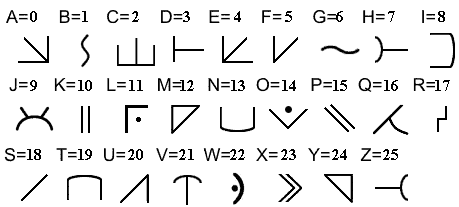
\includegraphics[width=.5\textwidth]{autokey_chiffre.png}
\end{center}

\begin{longtable}{|r|c|c|c|c|c|c|c|c|c|c|c|c|}
\hline
Buchstabe & B & E &  N &  D &  E &  R &  O &  K\\\hline
Zahl      & 1 & 4 & 13 &  3 &  4 & 17 & 14 & 10\\\hline
Summe     & 1 & 5 & 18 & 21 & 25 & 42 & 56 & 66\\\hline
mod 26    & 1 & 5 & 18 & 21 & 25 & 16 &  4 & 14\\\hline
\end{longtable}

\begin{center}
	
\includegraphics[width=.4\textwidth]{bender_ok.png}
\end{center}

\end{frame}

\begin{frame}
\frametitle{Autokey-Chiffre}
\begin{block}{Definition:}
\begin{itemize}
	\item Basiert auf Vigenère-Chiffre
	\item Ist Schlüsselwort kürzer als Klartext, wird Klartext an Schlüsselwort angehängt
	\item Stand der Technik im 16. Jahrhundert
\end{itemize}
\end{block}
\end{frame}



\section{IT}

\subsection{Hardware}

\frame{
\frametitle{Computer}
\begin{block}{Volksabstimmung in Springfield}
\begin{itemize}
	\item Apu hat bei Prof. Dr. Frink am SHIT\footnote{Springfield Heights Institute of Technology} Informatik studiert
	\item Prof. Dr. Frink behauptet:
	\begin{itemize}
		\item In weniger als 100 Jahren sind Computer doppelt so leistungsfähig
		\item 1000-mal größer
		\item So teuer, dass nur die fünf reichsten Könige Europas diese sich leisten können
	\end{itemize}
\end{itemize}
\end{block}
}

\frame{
\only<presentation>{
	\frametitle{Computer}
}
\begin{block}{Mooresches Gesetz}
\begin{itemize}
	\item Geht auf Gordon Moore, einen Mitbegründer von Intel zurück
	\item Die Zahl der Transistoren von integrierten Schaltungen (IC) verdoppelt sich jährlich
	\item Heute geht man davon aus, dass der Zeitraum der Verdoppelung mit 18 Monaten hinreichend genau erfasst ist
\end{itemize}
\end{block}
}

\only<article>{
  \newpage
}
\subsection{Programmiersprachen}

\frame{
\only<presentation>{
	\frametitle{Fortran}
}
\begin{block}{Der Mann, der als Dinner kam}
\begin{itemize}
	\item Simpsons werden auf den Planeten Riegel 7 entführt
	\item Bewohner des Planeten behaupten, Fortran sei die beste Programmiersprache
	\item Fortran gilt als die erste jemals tatsächlich realisierte höhere Programmiersprache
	\item Fortran geht auf Vorschlag aus 1953 von John Backus zurück
\end{itemize}
\end{block}
}

\begin{frame}
\only<presentation>{
	\frametitle{Fortran}
}
\begin{figure}[ht]
	\centering
	\only<presentation>{
		
\includegraphics[width=.75\textwidth]{old_fortran.png}
	}
	\only<article>{
	  
\includegraphics[width=.6\textwidth]{old_fortran.png}
	}
\end{figure}
\scriptsize{Quelle: \href{http://www.conquermaths.com/news/images/futfortran.jpg}{\url{http://www.conquermaths.com/news/images/futfortran.jpg}}}
\end{frame}

\begin{frame}[fragile]
\frametitle{BASIC}
\begin{block}{Wohnungssuche in Neu-New York}
\begin{itemize}
	\item Fry beschließt, bei Bender einzuziehen
	\item In Benders Wohnung hängt Stickbild mit folgendem Text:
\end{itemize}
\begin{lstlisting}[style=base]
@10@ HOME
@20@ SWEET
@30@ GOTO 10
\end{lstlisting}
\end{block}
\end{frame}

\subsection{Komplexitätstheorie}
\frame{
\only<presentation>{
	\frametitle{Komplexitätstheorie}
}
\begin{block}{$\mbox{Homer}^3$}
Es wird behauptet, dass Folgendes gilt:
\[P = NP\]
\end{block}
}

\frame{
\frametitle{P-NP-Problem}
\begin{block}{}
\begin{itemize}
	\item In welcher Beziehung stehen Komplexitätsklassen $P$ und $NP$ zueinander
	\begin{itemize}
		\item $P$: polynomial
		\item $NP$: nichtdeterministisch polynomial
	\end{itemize}
	\item Eines der wichtigsten ungelösten Probleme der Informatik
	\only<presentation>{
		\item Vom \href{http://www.claymath.org/}{Clay Mathematics Institute} in die Liste der Millennium-Probleme aufgenommen
	}
	\only<article>{
		\item Vom \href{http://www.claymath.org/}{Clay Mathematics Institute} in die Liste der Millennium-Probleme aufgenommen \cite{COO}
	}
\end{itemize}
\end{block}
}

\note{
\begin{itemize}
	\item Probleme der Klasse $P$ lassen sich einfach lösen (z.B. Multiplikation)
	\item Probleme der Klasse $NP$ sind schwer lösbar, aber leicht zu verifizieren (z.B. Zerlegung in Primfaktoren)
\end{itemize}
}

\subsection{Internet}

\frame{
\frametitle{Der blöde Uno-Club}
\begin{block}{Start-Up}
\begin{itemize}
	\item Homer gründet die Firma Compu-Global-Hyper-Mega-Net
	\item Hauptsitz ist das Esszimmer in der 742 Evergreen Terrace
	\item Einziger Kunde ist der Comic-Buchverkäufer
	\begin{itemize}
		\item  Will seine 28,8 Kilobaud Leitung zu einer 1,5 MBit-Fiber-Optic-T1-Leitung upgraden
		\item Benötigt einen IP-Router, der mit seiner Token-Ring-Ethernet-LAN-Konfiguration kompatibel ist
	\end{itemize}
	\item Bill Gates will anscheinend die Firma übernehmen, lässt aber die Zentrale zerstören
	\item Siehe \href{https://www.youtube.com/watch?v=KSKBRWoGvL0}{\url{https://www.youtube.com/watch?v=KSKBRWoGvL0}}
\end{itemize}
\end{block}
}

\note{
\begin{itemize}
	\item Originaltitel der Folge \grqq Das Bus\grqq
	\item Zitat Comic Book Guy:
	\begin{quotation}
		\glqq I'm interested in upgrading my 28.8 kilobaud Internet connection to an 1.5 megabit fiber optic T1 line. Will you be able to provide an IP router that's compatible with my token ring Ethernet LAN configuration?\grqq\
	\end{quotation}
	\item Neben der Folge mit dem deutschen Titel \grqq Das Bus\grqq\ gibt es noch die Folge \grqq Burns Verkaufen der Kraftwerk\grqq\ aus der dritten Staffel.
\end{itemize}
}

\frame{
\frametitle{Token Passing}
\begin{block}{Definition:}
\begin{itemize}
	\item Auf Deutsch auch als Token-Weitergabe bezeichnet
	\item Grundprinzip ist die kollisionsfreie Übertragung der Datenpakete zwischen den einzelnen Stationen
	\item Verwendet logisch die Ringtopologie
	\item Es existieren zwei unterschiedliche Realisierungsformen des Token Passing:
	\begin{itemize}
		\item Token Ring (IEEE 802.5) und
		\item Token Bus (IEEE 802.4)
	\end{itemize}
\end{itemize}
\end{block}
}

\frame{
\frametitle{Token Ring}
\begin{block}{}
\begin{center}
	\only<presentation>{
	\begin{tikzpicture}[scale=.85, every node/.style={scale=.85}]
	}
	\only<article>{
	\begin{tikzpicture}[scale=.9, every node/.style={scale=.9}]
	}
	\def \n {4}
\def \radius {3cm}
\def \margin {8}

\foreach \s in {1,...,\n}
{
	\node[draw, circle,very thick] at ({360/\n * (\s - 1)}:\radius) {$\s$};
	\draw[-,very thick] ({360/\n * (\s - 1)+\margin}:\radius) arc ({360/\n * (\s - 1)+\margin}:{360/\n * (\s)-\margin}:\radius);
}
\draw[->,color=blue,very thick] (-2,3.46) arc (120:150:4cm) node at (-3.7,2.83) {Token};
\end{tikzpicture}
\end{center}
\end{block}
}

\frame{
\frametitle{ISO/OSI-Basisreferenzmodell}
\tikzstyle{rechteck} = [rectangle split,minimum width=6cm, minimum height=1.5cm]
\begin{center}
	\only<presentation>{
	\begin{tikzpicture}[scale=.5, every node/.style={scale=.5}]
	}
	\only<article>{
	\begin{tikzpicture}[scale=.9, every node/.style={scale=.9}]
	}
	\node (17) at (0,9)    [rechteck, fill=blue!35] {};
\node at (0,9) {\small \textbf{Anwendungsschicht}};
\node (16) at (0,7.5)  [rechteck, fill=blue!30] {};
\node at (0,7.5) {\small \textbf{Darstellungsschicht}};
\node (15) at (0,6)    [rechteck, fill=blue!25] {};
\node at (0,6) {\small \textbf{Kommunikationssteuerungsschicht}};
\node (14) at (0,4.5)  [rechteck, fill=blue!20] {};
\node at (0,4.5) {\small \textbf{Transportschicht}};
\node (13) at (0,3)    [rechteck, fill=blue!15] {};
\node at (0,3) {\small \textbf{Vermittlungsschicht}};
\node (12) at (0,1.5) [rechteck, fill=blue!10] {};
\node at (0,1.6) {\parbox{6cm}{\centering \small \textbf{Sicherungsschicht}\\
  \footnotesize Logical Link Control\\
  \footnotesize \textbf{Media Access Control}}
};
\node (11) at (0,0)    [rechteck, fill=blue!5]  {};
\node at (0,0) {\small \textbf{Bit\"ubertragungsschicht}};

\node (27) at (8,9)    [rechteck, fill=blue!35] {};
\node at (8,9) {\small \textbf{Application Layer}};
\node (26) at (8,7.5)  [rechteck, fill=blue!30] {};
\node at (8,7.5) {\small \textbf{Presentation Layer}};
\node (25) at (8,6)    [rechteck, fill=blue!25] {};
\node at (8,6) {\small \textbf{Session Layer}};
\node (24) at (8,4.5)  [rechteck, fill=blue!20] {};
\node at (8,4.5) {\small \textbf{Transport Layer}};
\node (23) at (8,3)    [rechteck, fill=blue!15] {};
\node at (8,3) {\small \textbf{Network Layer}};
\node (22) at (8,1.5) [rechteck, fill=blue!10] {};
\node at (8,1.6) {\parbox{6cm}{\centering \small \textbf{Data Link Layer}\\
  \footnotesize Logical Link Control Sublayer\\
  \footnotesize \textbf{Media Access Control Sublayer}}
};
\node (21) at (8,0) [rechteck, fill=blue!5] {};
\node at (8,0) {\small \textbf{Physical Layer}};

\draw[<->,thick,dashed] (17) -- (27);
\draw[<->,thick,dashed] (16) -- (26);
\draw[<->,thick,dashed] (15) -- (25);
\draw[<->,thick,dashed] (14) -- (24);
\draw[<->,thick,dashed] (13) -- (23);
\draw[<->,thick,dashed] (12) -- (22);
\draw[<->,thick,dashed] (11) -- (21);

\node at (4,.25)  {1};
\node at (4,1.75) {2};
\node at (4,3.25) {3};
\node at (4,4.75) {4};
\node at (4,6.25) {5};
\node at (4,7.75) {6};
\node at (4,9.25) {7};

\draw[<->,thick] (-3.5,9) -- (-3.5,-1.25) -- (11.5,-1.25) -- (11.5,9);

\draw[<->,thick,dashed] (-2.5,-2) -- (2.5,-2);
\node at (0,-1.75) {\small Virtuelle Protokolle der Schichten};
\draw[<->,thick,] (5.5,-2) -- (10.5,-2); 
\node at (8,-1.75) {\small Tats\"achlicher Transport};
\end{tikzpicture}
\end{center}
}

\frame{
\frametitle{Zitate Homer}
\begin{block}{}
\begin{quote}
	\grqq Internet! Is that thing still around?\grqq
\end{quote}
\begin{quote}
	\grqq The internet wasn't created for mockery, it was supposed to help researchers at different universities share data sets. It was!\grqq
\end{quote}
\begin{quote}
	\grqq Kids are great. You can teach them to hate what you hate and, with the Internet and all, they practically raise themselves.\grqq
\end{quote}
\end{block}
}

\subsection{IT-Sicherheit}

\frame{
\only<presentation>{
	\frametitle{IT-Sicherheit}
}
\begin{block}{Benders Big Score}
\begin{itemize}
	\item Dr. Zoidberg wird Opfer eines Vorschussbetrugs (Nigerian Scam)
	\item Prof. Farnworth hat in der spanischen Lotterie gewonnen, obwohl er kein Los gekauft hat
	\item Bender glaubt einer Werbung, dass er durch Schauen von Erwachsenenfilmen reich werden kann
	\item Generelle Leichtgläubigkeit im Umgang mit persönlichen Daten (z.B. Kreditkartennummer)
\end{itemize}
\end{block}
}

\frame{
\only<presentation>{
	\frametitle{IT-Sicherheit}
}
\begin{block}{Ein Herz und eine Krone}
\begin{itemize}
	\item Moe wird Opfer des Nigerian Scam
	\item Als sich echte nigerianische Prinzessin in sein Lokal verirrt, will er von ihr das Geld zurück
\end{itemize}
\end{block}
}

\section{Quantenphysik}

\subsection{Heisenberg}

\frame{
\only<presentation>{
	\frametitle{Heisenbergsche Unschärferelation}
}
\begin{block}{Das Glück des Phillip J. Fry}
\begin{itemize}
	\item Beim Pferderennen beschwert sich Professor Farnsworth über das Ergebnis eines Quantumzieleinlaufs
	\item Ergebnis sei durch Messung verfälscht worden
\end{itemize}
\end{block}
}

\frame{
\only<presentation>{
	\frametitle{Heisenbergsche Unschärferelation}
}
\begin{block}{Definition:}
\begin{itemize}
	\item Komplementäre Eigenschaften eines Teilchens sind nicht gleichzeitig beliebig genau bestimmbar
	\item Beispiel: Ort und Impuls
\end{itemize}
	\[\Delta x \cdot \Delta p \geq \frac{h}{2\pi}
\]
\end{block}
}

\note{
\begin{itemize}
	\item Besitzt ein Körper der Masse $m$ die Geschwindigkeit $\vec{v}$ , so definiert man als Impuls des Körpers den Vektor
\end{itemize}
	\[
	\vec{p} = m\cdot \vec{v}
\]
}

\subsection{Schrödinger}

\frame{
\only<presentation>{
	\frametitle{Quantenphysik}
}
\begin{block}{Law and Oracle}
\begin{itemize}
	\item Erwin Schrödinger wird von der Polizei aufgehalten, weil er mit fünf Meilen pro Stunde schneller als Lichtgeschwindigkeit unterwegs war
	\item Nachdem ihn die Polizei aufgehalten hat, will er nicht sagen, was sich in der Kiste auf dem Beifahrersitz befindet
	\item Fry öffnet die Kiste und eine Katze springt ihn an
\end{itemize}
\end{block}
}

\frame{
\frametitle{Schrödingers Katze}
\begin{block}{}
\begin{itemize}
	\item Gedankenexperiment zur Überlagerung von Zuständen in der Quantenmechanik
	\item Superposition der Zustände
\end{itemize}
\end{block}
}

\note{
\begin{itemize}
  \item Schrödingers Gedankenexperiment wird auch in der Serie \glqq The Big Bang Theory\grqq\ erwähnt.
  \item Hier wird dabei der Status der Beziehung zwischen Penny und Leonard thematisiert.
\end{itemize}
}

\frame{
\frametitle{Schrödingergleichung}
\begin{block}{Definition:}
Schrödingergleichung in ihrer allgemeinsten Form lautet:
\begin{displaymath}
i\hbar \frac{\partial \Psi}{\partial t} = -\frac{\hbar^2}{2m}
\frac{\partial^2 \Psi}{\partial x^2} + V \Psi
\end{displaymath}
\end{block}
}

\section{Literaturverzeichnis}
\frame{
\only<presentation>{
	\frametitle{Literaturverzeichnis}

\begin{thebibliography}{99999}
	\bibitem[FLI]{MF} Markus Flingelli: \textit{Hier sind die Simpsons}, 12. überarbeitete Ausgabe, 27. Oktober 2019, \href{https://github.com/mflingelli/simpsons/releases/download/v12.0/Simpsons.pdf}{\url{https://github.com/mflingelli/simpsons/releases/download/v12.0/Simpsons.pdf}}
	\bibitem[GGW]{GG} Tom Georgoulias, Sarah J. Greenwald und Marc Wichterich: \textit{Futurama $\pi$k -- Mathematics in the year 3000}, Math Horizons, Volume 11, Number 4, April 2004, pp. 12-15
	\bibitem[GRE]{SG} Sarah J. Greenwald: \textit{Klein's Beer: Futurama Comedy and Writers in the Classroom}, 2007
	\bibitem[SIN]{SS} Simon Singh: \textit{Homers letzter Satz}, Carl Hanser Verlag, München, 2013
\end{thebibliography}
}
\only<article>{
\begin{thebibliography}{99999}
  \bibitem[BBC]{BBC} BBC News: \textit{Glasgow University offers Homer Simpson philosophy class}, 16. November 2016, \href{http://www.bbc.com/news/uk-scotland-glasgow-west-37999573}{\url{http://www.bbc.com/news/uk-scotland-glasgow-west-37999573}}
  \bibitem[BOE]{BOE} Harald Bögeholz: \textit{Zahlen, bitte! Fermats letzter Satz, Andrew Wiles und die Simpsons}, heise online, 11. April 2017, \href{https://www.heise.de/newsticker/meldung/Zahlen-bitte-Fermats-letzter-Satz-Andrew-Wiles-und-die-Simpsons-3678787.html}{\url{https://www.heise.de/newsticker/meldung/Zahlen-bitte-Fermats-letzter-Satz-Andrew-Wiles-und-die-Simpsons-3678787.html}}
  \bibitem[COO]{COO} Stephen Cook: \textit{The P versus NP problem}, \href{http://www.claymath.org/sites/default/files/pvsnp.pdf}{\url{http://www.claymath.org/sites/default/files/pvsnp.pdf}}
  \bibitem[FIS]{FIS} Sebastian Fischer: \textit{Stoibers Glaubensgipfel}, Spiegel Online, Juni 2006, \href{http://www.spiegel.de/politik/deutschland/0,1518,419948,00.html}{\url{http://springfield-shopper.de/Information/whoiswho_bewohner.shtml}}
  \bibitem[FLI]{MF} Markus Flingelli: \textit{Hier sind die Simpsons}, 12. überarbeitete Ausgabe, 27. Oktober 2019, \href{https://github.com/mflingelli/simpsons/releases/download/v12.0/Simpsons.pdf}{\url{https://github.com/mflingelli/simpsons/releases/download/v12.0/Simpsons.pdf}}
  \bibitem[GGW]{GG} Tom Georgoulias, Sarah J. Greenwald und Marc Wichterich: \textit{Futurama $\pi$k -- Mathematics in the year 3000}, Math Horizons, Volume 11, Number 4, April 2004, pp. 12-15
  \bibitem[GRE]{SG} Sarah J. Greenwald: \textit{Klein's Beer: Futurama Comedy and Writers in the Classroom}, 2007
  \bibitem[SIN]{SS} Simon Singh: \textit{Homers letzter Satz}, Carl Hanser Verlag, München, 2013
  \bibitem[ZOT]{ZOT} Volker Zota: \textit{Zahlen, bitte! 1729 -- was Taxis mit Futurama zu tun haben}, heise online, 22. November 2017, \href{https://www.heise.de/newsticker/meldung/Zahlen-bitte-1729-was-Taxis-mit-Futurama-zu-tun-haben-3492957.html}{\url{https://www.heise.de/newsticker/meldung/Zahlen-bitte-1729-was-Taxis-mit-Futurama-zu-tun-haben-3492957.html}}
\end{thebibliography}
}
}

\only<presentation>{
\begin{frame}
	\frametitle{Fragen?}
	\begin{figure}[ht]
		\centering
		
\includegraphics[height=.75\textheight]{homer_pythagoras.png}
	\end{figure}
	\scriptsize{Quelle: \href{https://vividkaret.files.wordpress.com/2014/10/homer.png}{\url{https://vividkaret.files.wordpress.com/2014/10/homer.png}}}
\end{frame}
}

\end{document}